
In this section we will define a procedure, which will be called elastic
registration, to perform a groupwise alignment of a dataset under this
framework. A target function will be created, called elastic mean, to which all
samples will be aligned later, as discussed in section \ref{SEC:L2PAIRWISE}.

Let $\{f_i\} \subset \mathscr{F}$ be a dataset of functions to register and
$q_i$ their corresponding SRSFs. Firstly we will compute their Karcher mean in
$\mathscr{A}$, defined as

\begin{equation}[]{Karcher mean on $\mathscr{A}$}
\left[\mu_{q}\right]=\underset{[q] \in \mathscr{A}}{\operatorname{arginf}}
\sum_{i=1}^{n} d_{a}\left([q],\left[q_{i}\right]\right)^{2}.
\end{equation}

The bracket notation $[\mu_{q}]$ is used to emphasize the fact it is an orbit in
a quotient space. We will need a criterion to select a particular element of
this orbit, for that reason we will define the center of the orbit as the
element $\tilde \mu_{q}  \in [\mu_{q}]$  such that the relatives phases
${\gamma_i^*}$ between ${q_i}$ and $[\mu_{q}]$ have as Karcher mean the identity.

We will select an arbitrary element $\mu_{q}$ of $[\mu_{q}]$ to which we will
calculate the corresponding warping functions to align the set of SRSFs, i.e.,
$\gamma_{i}=\operatorname{arginf}_{\gamma \in \Gamma}\left\|\tilde{q}-
\left(q_{i}, \gamma\right)\right\|$.

\begin{figure}[Scheme of the elastic registration procedure]{FIG:SCHEME}{Scheme of the elastic registration procedure.}
  \includegraphics[width=6cm]scheme-elastic}
\end{figure}

Then, we will compute the Karcher mean of $\{\gamma_i\}$, denoted as
$\bar \gamma$, in the phase space, using the algorithm detailed in the
appendix B.3. The center of the orbit will be
$\tilde \mu_q = (\mu_q , {\bar \gamma}^{-1})$.

The mean of the relative phases with respect to $\tilde \mu_q$, will be the
identity, thus

\begin{equation}[]{Identity mean}
%\bar {\{  \gamma_i \circ {\bar \gamma}^{-1}  \}} =
\operatorname{arginf}_{\gamma \in \Gamma}d_{FR}(\gamma_i \circ {\bar \gamma}^{-1}, \gamma) =
\operatorname{arginf}_{\gamma \in \Gamma}d_{FR}(\gamma_i \circ {\bar \gamma}^{-1} \circ \bar \gamma, \gamma \circ \bar \gamma) =
\operatorname{arginf}_{\gamma \in \Gamma}d_{FR}(\gamma_i, \gamma \circ \bar \gamma) = \gamma_{id}.
\end{equation}

Finally, we will construct the template to which the samples will be aligned,
called elastic mean,
$\tilde \mu_f = \frac{1}{N} \sum_{i=1}^N f_i(0) +
\int_0^t \tilde \mu_q(s) | \tilde \mu_q(s)| ds$,
which is the pullback of $\tilde \mu_q$ to the original space $\mathscr{F}$. In
the figure \ref{FIG:ELASTICREG} may be observed the result of the registration of the
berkeley growth curves of the figure \ref{FIG:BERKELEY}.

\begin{figure}[Elastic registration of the Berkeley velocity curves]{FIG:ELASTICREG}{Elastic registration of the Berkeley velocity curves}
  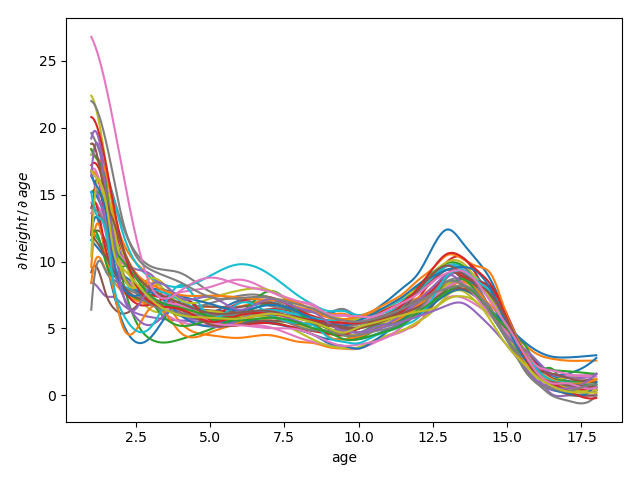
\includegraphics[width=8cm]{berkeley-registered}
\end{figure}

An important property of the elastic mean
$\tilde \mu_f$ is that given a dataset $\{c_i f(\gamma_i(t)) + e_i\}_{i=1}^{n}$, where
$\{\gamma_i\}_{i=1}^{n}$ have as Karcher mean in $\Gamma$ the identity and $c_i$ and $e_i$ are positive
constants with mean $1$ and $0$ respectively, then $\tilde \mu_f$ is a
consistent estimator of $f$ [refff to paper].
